
% archiIllustrrate
\begin{comment}
\begin{figure}[hb]
\centering
% 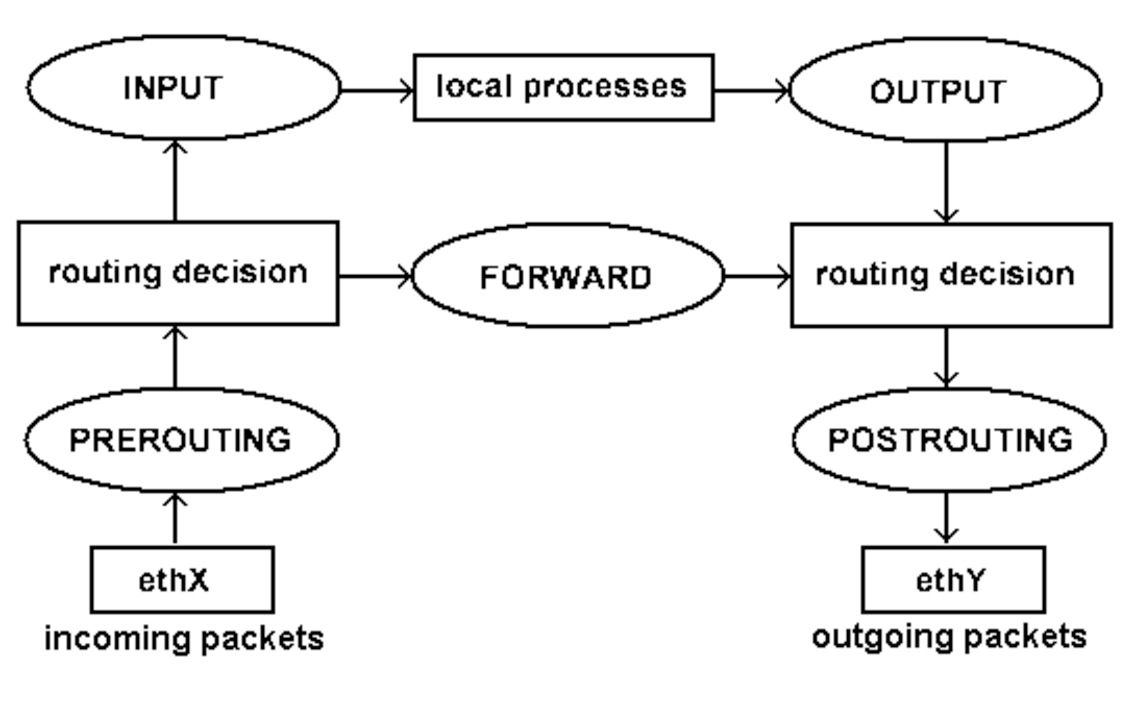
\includegraphics[scale=0.25]{figures/netfilter.pdf} 
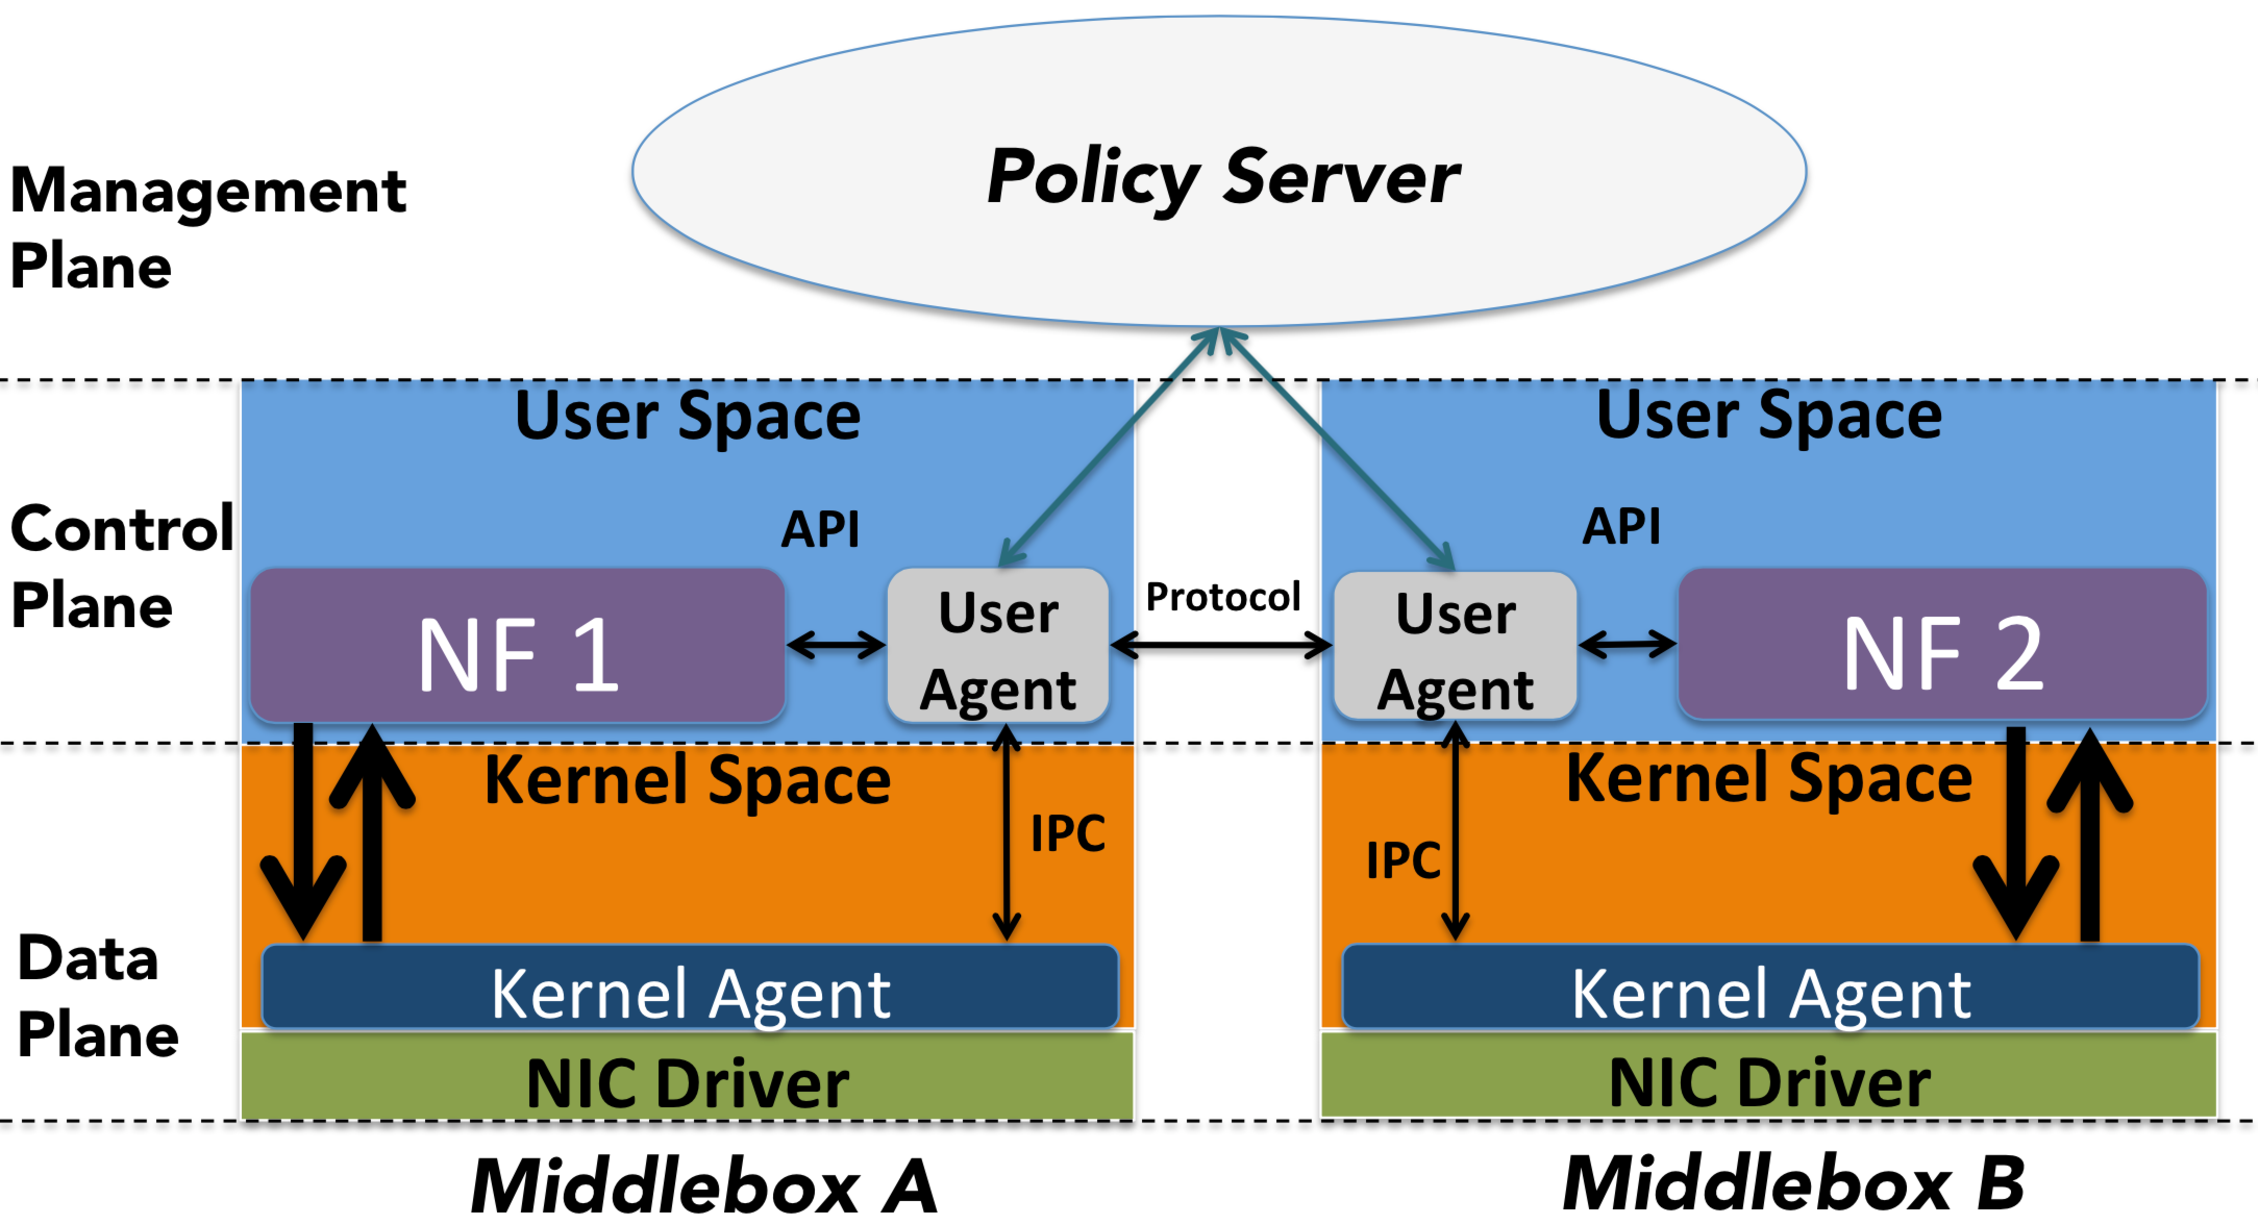
\includegraphics[width=\linewidth]{figures/archiIllustrrate.pdf} 

\caption{\small Middlebox protocol architecture}\label{expTopo}
\end{figure}
\end{comment}

\section{Protocol}
\label{sec:protocol}
\begin{comment}
We explain the basic indirection protocol in subsection~\ref{basic}, a three-way handshake that exchanges state enabling future migration in subsection~\ref{twoway}, and a migration protocol in subsection~\ref{mobile}. The middlebox-aware session protocol can: (i) successfully establish a connection through the two-way handshake; (ii) support a flexible migration of either endhosts or middleboxes; and (iii) gracefully close the connection, or sub-sessions during the migration. 
\end{comment}

Considering middleboxes as explicit components of the end-to-end between two endpoints is the crux of our protocol. Only by doing so can we achieve the desired scalability and flexibility for both endpoints and middleboxes. We discuss session setup in \S\ref{setup} and flow migration control in \S\ref{MigrateLogic}.  

\subsection{Session Setup}\label{setup}

In \system protocol, each endpoint or middlebox sends packets whose destination is the next middlebox or endpoint in the session path. This obviates the need for special support in the switch or router to direct packets through the chosen chain of network functions (service chain), despite changes in network topology or host movement. 

The list of middleboxes, $L$, that a flow has to traverse is provided by the policy server and can be pulled from the server or pushed to the client. When the client initiates the connection, the control plane uses a three-way handshake to establish the supersession and its associated subsessions. More specifically, the client's control plane sends a SYN message to the first middlebox that includes the supersession header and $L$. The middlebox strips itself from the head of $L$, gets the address of the next middlebox from $L$, and relays the rest of the message to the next middlebox. The SYN message is thus passed recursively through the elements of $L$ before reaching the server. Upon receiving the SYN, the server sends a SYNACK back to the client using $reverse(L)$. Upon receiving the SYNACK, the client immediately sends an ACK to the server via the same mechanism. Once these three control messages are exchanged, the supersession and subsessions are established, and data packets are explicitly addressed to the subsession IPs.

If we simply rewrite the source and destination IPs, we lose supersession information and introduce ambiguity. Consider the case where flow \textit{a} and \textit{b} have the same source port and destination IP and port, but different source IPs. If \textit{a} and \textit{b} share the same first hop middlebox, the two flows may become indistinguishable upon arrival at the first hop middlebox. To address this issue, we modify the port numbers to identify the flow, a standard technique in NAT~\cite{NAT}. We integrate this port allocation into the three-way handshake: port mappings are assigned in a middlebox when it receives a SYN, and initiates a new subsession with the rewritten port numbers. If we rewrite both source and destination ports, \system can support four billion unique flows per middlebox pair. See Figure~\ref{sessionsetup} for the complete session setup.

\begin{figure}[ht]
\centering
% 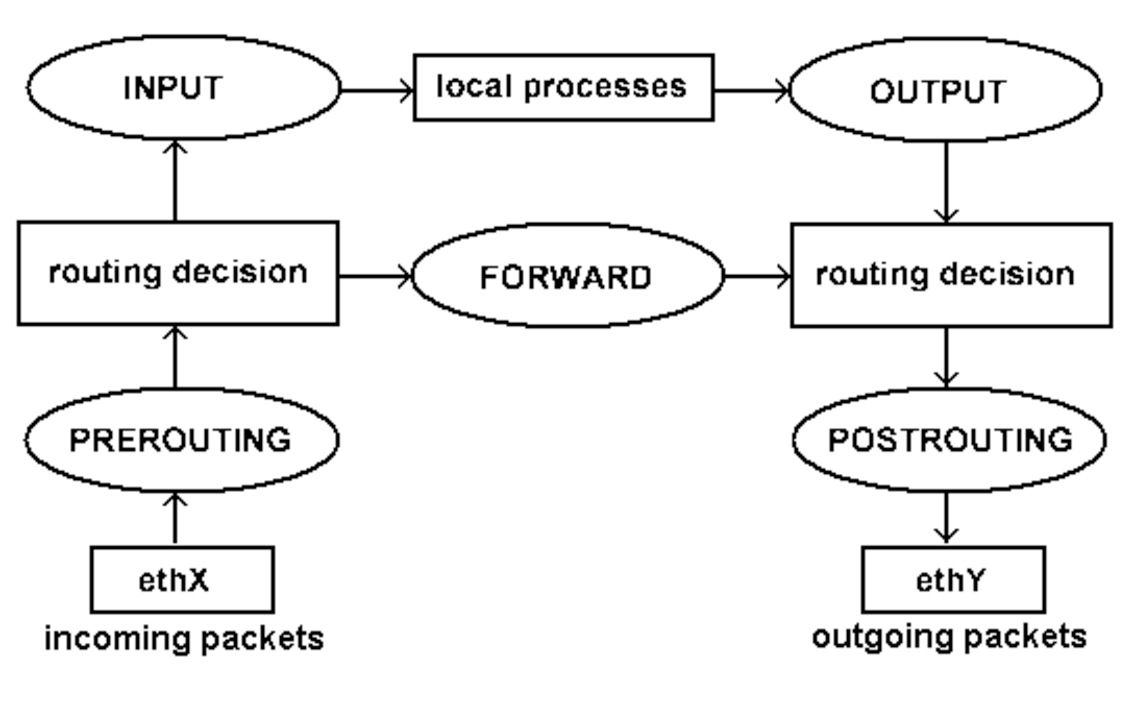
\includegraphics[scale=0.25]{figures/netfilter.pdf} 
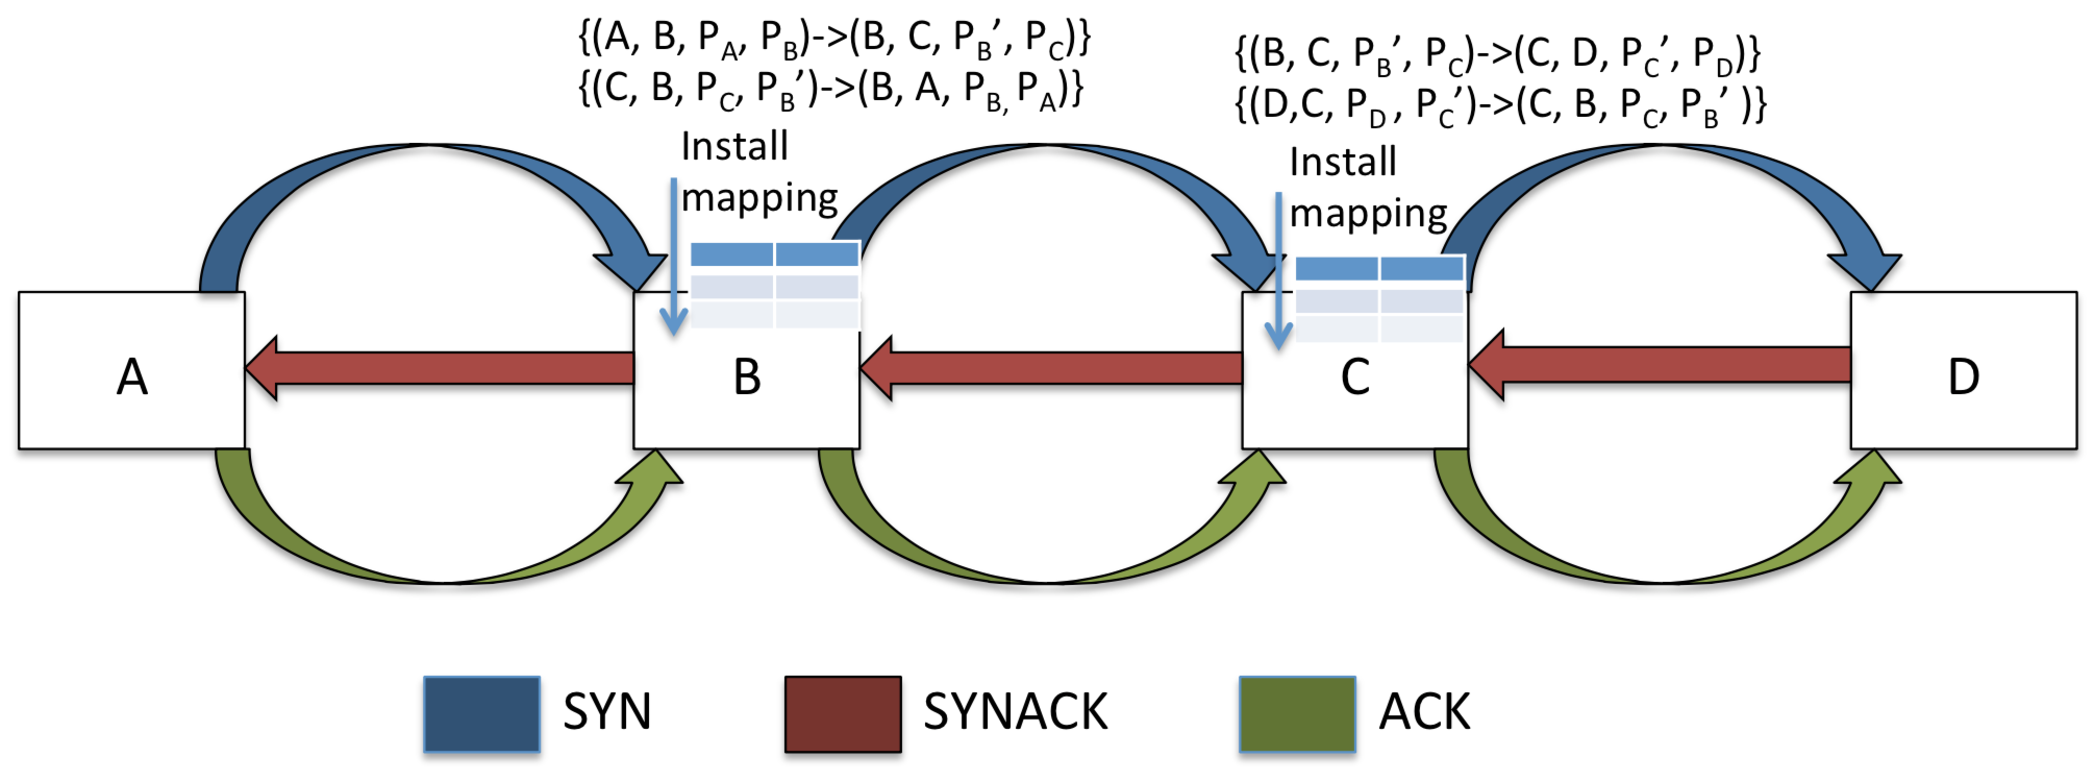
\includegraphics[width=\linewidth]{figures/threeway.pdf} 

\caption{\small  Session setup}\label{sessionsetup}
\end{figure}



\subsection{Migration and Mobility Control}\label{MigrateLogic}
%Dynamic network function policies are gaining ground today because of the flexibility they offer. 

Supporting dynamic middlebox modification for a flow improves the efficiency of the network and NF use, e.g. --- removing a cache proxy if the content is not cache-able, inserting an IDS upon detecting suspicious flows, or switching from a heavily loaded transcoder to a lightly loaded one. As a natural extension of general middlebox migration, we also include endhost mobility in the design of \system; supporting mobility is also critical in cellular networks.

\subsubsection{``Make before break''} \label{migration1}
To find the right mechanism to support flow migration, we investigated existing mobility protocols~\cite{TCPMobile, I3Mobile, mip, serval, lisp, hip} under the session-location mobility framework~\cite{zave}. However, the key distinction between host mobility and NF flow migration is that a move in host mobility is unexpected, whereas flow migration among middleboxes is planned (or controlled?). 

In fact, this type of reconfiguration is quite common in circuit design and addressed via the ``make before break'' philosophy. Namely, we stitch together subsessions on the new path before closing the subsessions on the old path. To achieve this, we treat the two neighbors of the moving middlebox as two \textit{signaling endpoints} during a flow migration. We stress that the resulting three nodes that are involved in the migration are \textit{consecutive}. Because we offload some policy decisions to the middleboxes, this property ensures that a middlebox cannot decide the fate of other on-path middleboxes that are not directly affected by the migration. 

For a middlebox insertion, we first identify and notify one of the two \textit{signaling endpoints} as an initiating point in a deterministic way. We start from the initiating point, set the two \textit{signaling endpoints} in a suspend state for data transfer for the new path, and complete a three-way handshake (UPDATE-SYN, UPDATE-SYNACK and UPDATE-ACK) on a new path that includes the two \textit{signaling endpoints} and the new middlebox to insert, to ensure the path establishment. Once the new path is established, we start the data transfer on the new path and remove the old path. We extend the same mechanism to handle middlebox removal and replacement. 

\subsubsection{Handling Concurrent Migration}
When we offload dynamic network function policy to a distributed control plane, we expect cases where two middleboxes initiate simultaneous move operations. In particular, if two neighbor middleboxes both initiate removal, we may lose the supersession connection. Strawman solutions include: (1) using a two phase commit to allow the one with the highest ID to move first; (2) a central controller that assigns token to the middleboxes. However, strong serialization via a two phase commit is not necessary, and a central controller suffers from scalability, thereby deviating from the initial design goal. We should furthermore allow concurrent moves at different points of the service chain. 

To address concurrent migration, we rely on the following properties: (i) migration is per flow, and (ii) at most three nodes on the current service chain are involved in each flow migration. The two assumptions help us design an efficient algorithm: migration can happen simultaneously for different flows, and concurrent migrations can happen at different points of the service chain if they involve disjoint sets of nodes; each node has a \texttt{pending} counter to ensure that it participates in at most one concurrent update.


Middleboxes for a flow have a strict ordering, which is simply the order in which the middleboxes are traversed by the path from the client to the server. We can define two comparators on this ordering, which we term ``left'' and ``right''. $M_{1}$ is left of $M_{2}$ iff the path from the client to $M_{2}$ passes through $M_{1}$; $M_{1}$ is right of $M_{2}$ iff the path from the client to $M_{1}$ passes through $M_{2}$. The proposed algorithm only allows one concurrent operation for all the nodes involved. When a migration is initiated at a certain node, the node postpones the update if its \texttt{pending} counter is not zero, otherwise it increments the \texttt{pending} counter and sends the request to the node immediately to its left if the migration is removal or replacement, or connects to the new middlebox if it is an insertion. If the left side responds with a reject, the node backs off, otherwise it receives an approval and proceeds with the update. A node always accepts UPDATE-SYN requests (establishing a new path). Algorithm~\ref{concurrency} describes the algorithm details and Figure~\ref{concurfigure} depicts the steps for migrations.


\begin{figure}[ht]
\centering
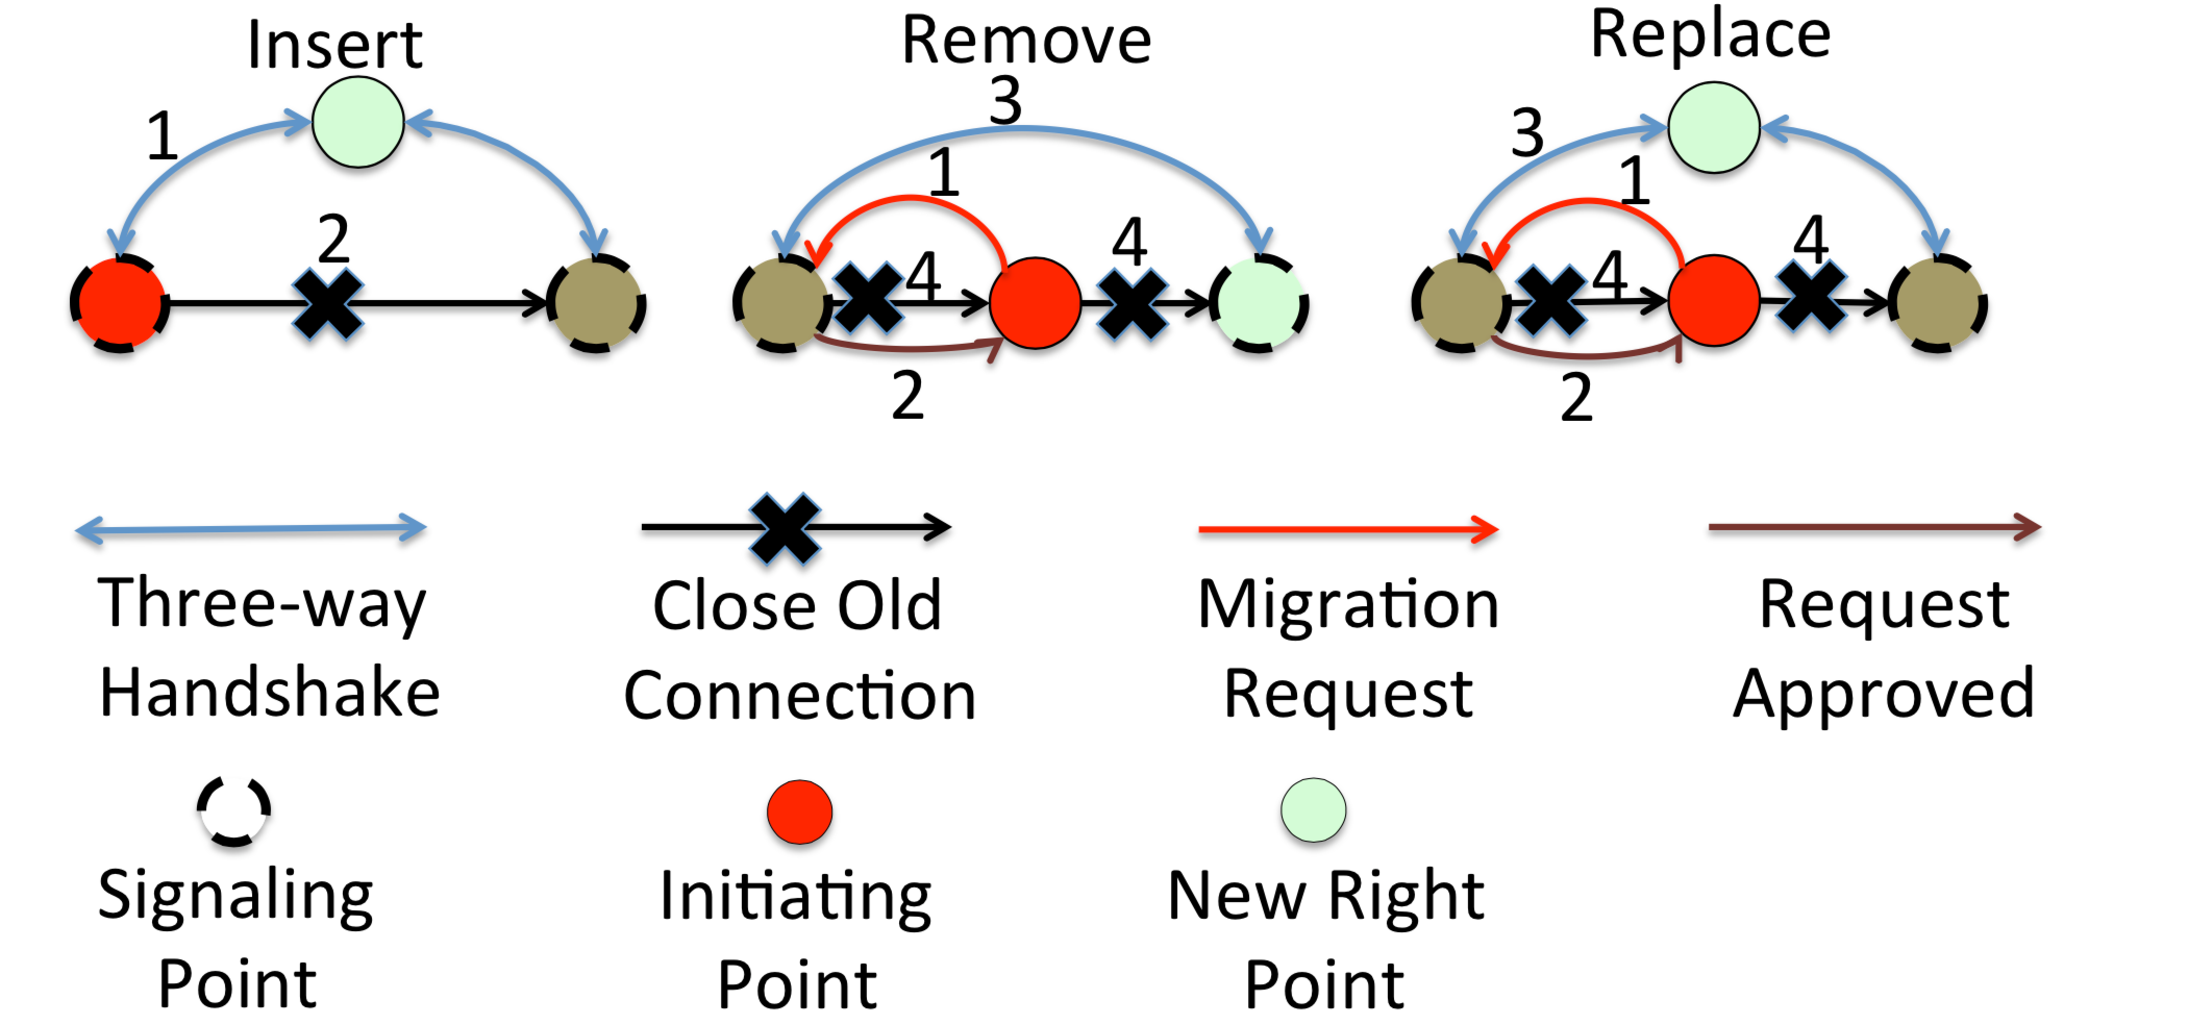
\includegraphics[width=\linewidth]{figures/concurrentupdate.pdf} 
\caption{\small Flow migration during insert, remove and replace}\label{concurfigure}
\end{figure}


\begin{algorithm} [htb]
%\small
\scriptsize

\SetAlgoLined

\SetKwFunction{update}{Trigger\_Migration}\SetKwFunction{IPC}{Msg\_Handler }\SetKwFunction{queue}{Queue Agent}
\SetKwProg{func}{Function}{}{}

\func{\update{} } {
\If{recv(migrate)}
{
  \If{pending == 0} {
  pending++\;
  \If{migration == insert }{
    sendto(New right, UPDATE-SYN)\;
   
  } \Else{
   sendto(Left, request)\;
  }
  }
  \Else{
  Exponentially backoff and retry\;
  }
}


}
\func{ \IPC{} }{
\If{recv(request)}{
  \If{pending$>0$ }{
  sendback(reject)\;
  }
  \Else{
  pending++ \;
  sendto(New right, UPDATE-SYN)\;
  sendback(approve)\;
  }
}

\If{recv(reject) }{
 Exponentially backoff and retry sendto(Left, request)\;
}
\If{recv(approve) }{
//do nothing, to avoid request re-transmission
}

\If{recv(UPDATE-SYN)}
{
  pending++\;
  \If{(migration==insert or replace) and (current == not signaling point) }{
    forward(UPDATE-SYN)\;
  }
  \Else{
  sendback(UPDATE-SYNACK)\;
  } 
  
}
\If{recv(close)}
{
  //clean old flow state\;
  pending$--$\;
}
\If{recv(UPDATE-SYNACK)}{
  pending$--$\;
  \If{(migration==insert or replace) and (current == not signaling point) }{
    forward(UPDATE-SYNACK)\;
  }
  \Else{
  sendto(OldMBox, close)\;
  sendback(UPDATE-ACK)\;
    //clean old flow state\
  } 
  
}
\If{recv(UPDATE-ACK)}{
  pending$--$\;
   \If{(migration==insert or replace) and (current == not signaling point) }{
    forward(UPDATE-ACK)\;
  } \Else{
    //clean old flow state\
  }
 
}

}
\caption{ Concurrent Flow Migration} \label{concurrency}

\end{algorithm} 


\subsubsection{``Break before make''}
When a client moves, it may drop the old subsession before establishing a new subsession. Consider when a UE moves across a cell boundary, upon which the UE may suffer from transient connection loss, since it is out of the old cell's range. 

After losing the old subsession, the client needs to rebind to the first hop middlebox. If we use the client's physical IP as part of the supersession identification, the first hop middlebox will fail to identify the supersession if the client changes its IP during mobility. To solve this problem, we can either put the old connection's information in the rebinding message sent by the client or, in a single domain case, administrators can assign a non-routeable IP to each device as a unique ID and use this ID to help identify the supersession. 
 
